\begin{frame}{Konstrukcija pravokotnice}
	\begin{columns}
	\begin{column}{0.55\textwidth}	
	\begin{itemize}[<+->]
		\item Dana sta premica \(p\) in točka \(T\).
		\item Nariši lok \(k\) s središčem v \(T\).
		\item Lok \(k\) seče premico \(p\) v točkah \(A\) in \(B\).
		\item Nariši lok \(m\) s središčem v \(A\).
		\item Nariši lok \(n\) s središčem v \(B\) in z enakim polmerom.
		\item Loka se sečeta v točki \(C\).
		\item Premica \(TC\) je pravokotna na \(p\).
	\end{itemize}
\end{column}

\begin{column}{0.45\textwidth}
	\only<1>{\centering 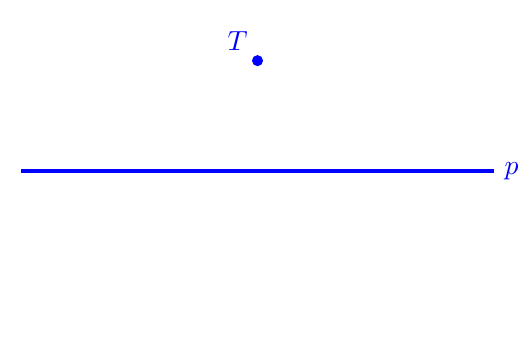
\includegraphics[width=50mm]{slike/fig-1.png}}
	\only<2>{\centering 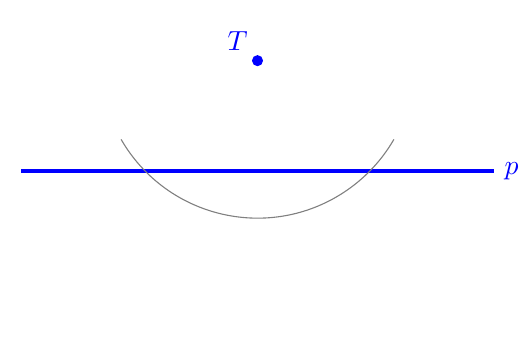
\includegraphics[width=50mm]{slike/fig-2.png}}
	\only<3>{\centering 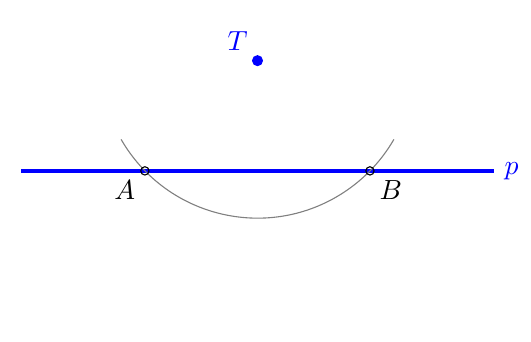
\includegraphics[width=50mm]{slike/fig-3.png}}
	\only<4>{\centering 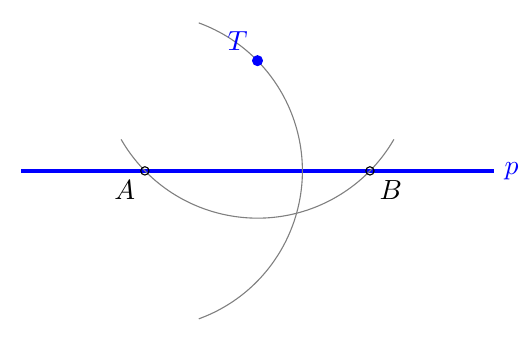
\includegraphics[width=50mm]{slike/fig-4.png}}
	\only<5>{\centering 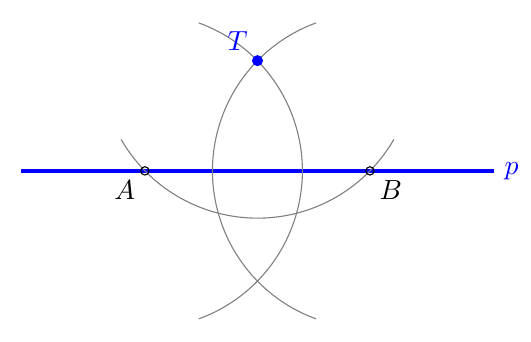
\includegraphics[width=50mm]{slike/fig-5.png}}
	\only<6>{\centering 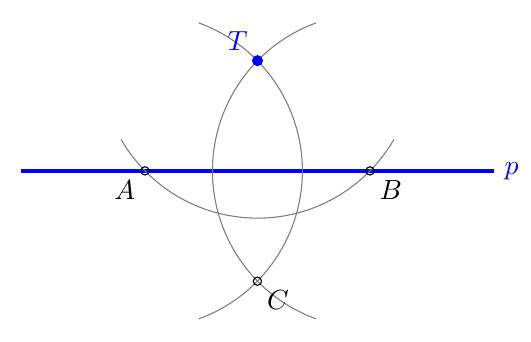
\includegraphics[width=50mm]{slike/fig-6.png}}
	\only<7>{\centering 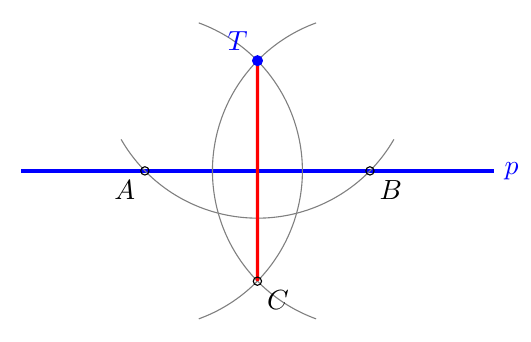
\includegraphics[width=50mm]{slike/fig-7.png}}
\end{column}
\end{columns}
\end{frame}
